% -*- coding:utf-8 -*-
\documentclass{standalone}
\usepackage{fontspec}
\setmainfont{Times New Roman}
\usepackage[UTF8]{ctex}
\usepackage{tikz}
\usepackage{amsmath}
\usetikzlibrary{matrix,calc,shapes,backgrounds,patterns,positioning,decorations.pathreplacing}
\begin{document}
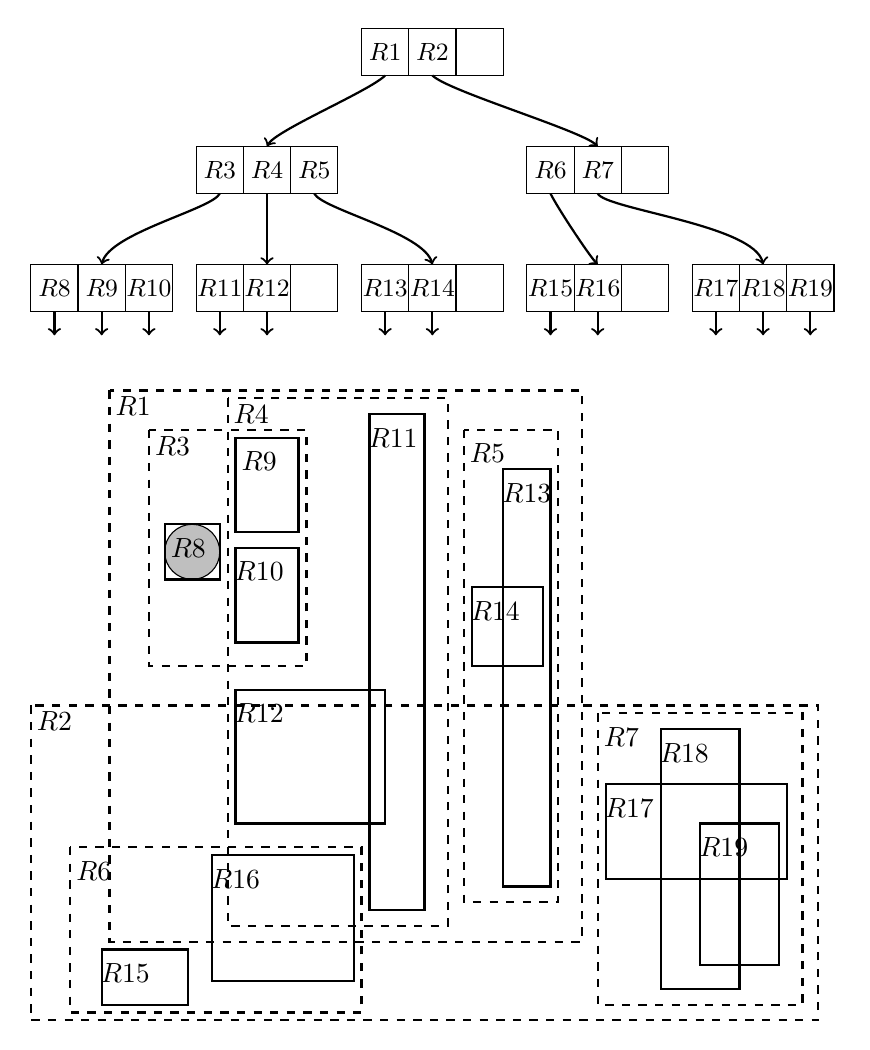
\begin{tikzpicture}
[
stepnode/.style={rectangle, rounded corners=0mm, draw=black, thick, align=center,width=0.5cm, height=0.5mm},
choicenode/.style={},
nodelabel/.style={font=\small},
dashrec/.style={rectangle, style=dashed,thick,},
]
%draw the bottom level
\draw (0,0) rectangle (0.6,0.6) node[nodelabel] at (0.3,0.3){$R8$};
\draw[thick, ->] (0.3,0) -- (0.3,-0.3);
\draw (0.6,0) rectangle (1.2,0.6) node[nodelabel] at (0.9,0.3){$R9$};
\draw[thick, ->] (0.9,0) -- (0.9,-0.3);
\draw (1.2,0) rectangle (1.8,0.6) node[nodelabel] at (1.5,0.3){$R10$};
\draw[thick, ->] (1.5,0) -- (1.5,-0.3);

\draw (0+2.1,0) rectangle (0.6+2.1,0.6) node[nodelabel] at (0.3+2.1,0.3){$R11$};
\draw[thick, ->] (2.4,0) -- (2.4,-0.3);
\draw (0.6+2.1,0) rectangle (1.2+2.1,0.6) node[nodelabel] at (0.9+2.1,0.3){$R12$};
\draw[thick, ->] (3,0) -- (3,-0.3);
\draw (1.2+2.1,0) rectangle (1.8+2.1,0.6) node[nodelabel] at (1.5+2.1,0.3){};

\draw (0+2.1+2.1,0) rectangle (0.6+2.1+2.1,0.6) node[nodelabel] at (0.3+2.1+2.1,0.3){$R13$};
\draw[thick, ->] (4.5,0) -- (4.5,-0.3);
\draw (0.6+2.1+2.1,0) rectangle (1.2+2.1+2.1,0.6) node[nodelabel] at (0.9+2.1+2.1,0.3){$R14$};
\draw[thick, ->] (5.1,0) -- (5.1,-0.3);
\draw (1.2+2.1+2.1,0) rectangle (1.8+2.1+2.1,0.6) node[nodelabel] at (1.5+2.1+2.1,0.3){};

\draw (0+2.1+2.1+2.1,0) rectangle (0.6+2.1+2.1+2.1,0.6) node[nodelabel] at (0.3+2.1+2.1+2.1,0.3){$R15$};
\draw[thick, ->] (6.6,0) -- (6.6,-0.3);
\draw (0.6+2.1+2.1+2.1,0) rectangle (1.2+2.1+2.1+2.1,0.6) node[nodelabel] at (0.9+2.1+2.1+2.1,0.3){$R16$};
\draw[thick, ->] (7.2,0) -- (7.2,-0.3);
\draw (1.2+2.1+2.1+2.1,0) rectangle (1.8+2.1+2.1+2.1,0.6) node[nodelabel] at (1.5+2.1+2.1+2.1,0.3){};

\draw (0+2.1+2.1+2.1+2.1,0) rectangle (0.6+2.1+2.1+2.1+2.1,0.6) node[nodelabel] at (0.3+2.1+2.1+2.1+2.1,0.3){$R17$};
\draw[thick, ->] (8.7,0) -- (8.7,-0.3);
\draw (0.6+2.1+2.1+2.1+2.1,0) rectangle (1.2+2.1+2.1+2.1+2.1,0.6) node[nodelabel] at (0.9+2.1+2.1+2.1+2.1,0.3){$R18$};
\draw[thick, ->] (9.3,0) -- (9.3,-0.3);
\draw (1.2+2.1+2.1+2.1+2.1,0) rectangle (1.8+2.1+2.1+2.1+2.1,0.6) node[nodelabel] at (1.5+2.1+2.1+2.1+2.1,0.3){$R19$};
\draw[thick, ->] (9.9,0) -- (9.9,-0.3);
%draw the middle level
\draw (2.1, 1.5) rectangle (2.7, 2.1) node[nodelabel] at (2.4, 1.8) {$R3$};
\draw (2.7, 1.5) rectangle (3.3, 2.1) node[nodelabel] at (3, 1.8) {$R4$};
\draw (3.3, 1.5) rectangle (3.9, 2.1) node[nodelabel] at (3.6, 1.8) {$R5$};

\draw (6.3, 1.5) rectangle (6.9, 2.1) node[nodelabel] at (6.6, 1.8) {$R6$};
\draw (6.9, 1.5) rectangle (7.5, 2.1) node[nodelabel] at (7.2, 1.8) {$R7$};
\draw (7.5, 1.5) rectangle (8.1, 2.1) node[nodelabel] at (7.8, 1.8) {};

\draw[thick, ->] (2.4,1.5) .. controls (2.3, 1.3) and (1, 1) .. (0.9,0.6);
\draw[thick, ->] (3, 1.5) -- (3, 0.6);
\draw[thick, ->] (3.6, 1.5) .. controls (3.7, 1.3) and (5,1) .. (5.1, 0.6);
\draw[thick, ->] (6.6, 1.5) .. controls (6.7, 1.3) and (7.1, 0.7) .. (7.2,0.6);
\draw[thick, ->] (7.2, 1.5) .. controls (7.3, 1.3) and (9.2,1.1) .. (9.3, 0.6);
%draw the top level
\draw (4.2, 3) rectangle (4.8, 3.6) node[nodelabel] at (4.5, 3.3){$R1$};
\draw (4.2+0.6, 3) rectangle (4.8+0.6, 3.6) node[nodelabel] at (4.5+0.6, 3.3){$R2$};
\draw (4.2+1.2, 3) rectangle (4.8+1.2, 3.6) node[nodelabel] at (4.5+1.2, 3.3){};
\draw[thick, ->] (4.5, 3) .. controls (4.3,2.8) and (3.1, 2.3) .. (3,2.1);
\draw[thick, ->] (5.1, 3) .. controls (5.3,2.8) and (7, 2.3) .. (7.2,2.1);

% draw the illustration
\draw[dashrec] (1,-1) rectangle (7, -8) node at (1.3, -1.2) {$R1$};
\draw[dashrec] (0,-5) rectangle (10, -9) node at (0.3, -5.2){$R2$};
\draw[dashrec] (1.5, -1.5) rectangle (3.5, -4.5) node at (1.8, -1.7){$R3$};
\draw[dashrec] (2.5, -1.1) rectangle (5.3, -7.8) node at (2.8, -1.3){$R4$};
\draw[thick][dashrec] (5.5, -1.5) rectangle (6.7, -7.5) node at (5.8, -1.8){$R5$};
\draw[fill=gray!50] (2.05, -3.05) circle (0.35);
\draw[thick] (1.7, -2.7) rectangle (2.4, -3.4) node at (2,-3){$R8$};
\draw[thick] (2.6, -1.6) rectangle (3.4, -2.8) node at (2.9, -1.9){$R9$};
\draw[thick] (2.6, -3) rectangle (3.4, -4.2) node at (2.9, -3.3){$R10$}; 
\draw[thick] (2.6, -4.8) rectangle (4.5, -6.5) node at (2.9, -5.1){$R12$};
\draw[thick] (4.3, -1.3) rectangle (5, -7.6) node at (4.6, -1.6){$R11$};
\draw[thick] (5.6, -3.5) rectangle (6.5, -4.5) node at (5.9, -3.8) {$R14$};
\draw[thick] (6, -2) rectangle (6.6, -7.3) node at (6.3, -2.3){$R13$};
\draw[dashrec] (0.5, -6.8) rectangle (4.2, -8.9) node at (0.8, -7.1) {$R6$};
\draw[thick] (0.9, -8.1) rectangle (2, -8.8) node at (1.2, -8.4){$R15$};
\draw[thick] (2.3, -6.9) rectangle (4.1, -8.5) node at (2.6, -7.2){$R16$};
\draw[dashrec] (7.2, -5.1) rectangle (9.8, -8.8) node at (7.5, -5.4){$R7$};
\draw[thick] (7.3, -6) rectangle (9.6, -7.2) node at (7.6, -6.3){$R17$};
\draw[thick] (8, -5.3) rectangle (9, -8.6) node at (8.3, -5.6){$R18$};
\draw[thick] (8.5, -6.5) rectangle (9.5, -8.3) node at (8.8, -6.8){$R19$};
\end{tikzpicture}
\end{document}